\chapter{Prior Work}\label{chap:prior_work}

\inline{
  Lots of past tense here --- where possible \& appropriate should probably be
  present.
}

An implementation of the main tool developed and used in this thesis,
``\pdsf{}'', predates the research presented in later chapters. As context for
the contributions in this thesis, this chapter will describe the state of the
project before the presented research was undertaken. Motivations for the tool's
original development are described in \cref{sec:pdsf_motivations}, which are
followed by its design and implementation in \cref{sec:prior_work_pdsf}, and
that of related tooling for experiments and simulations in
\cref{sec:prior_work_machinery}. The chapter concludes with a description of the
research undertaken using these tools in \cref{sec:caise_paper}, as some results
in the representation of behavioural variance using aspect orientation were
contributed using these tools which predate the research presented in later
chapters and offer important background for the research undertaken in it.

\section{Motivations in originally implementing \pdsf{}}\label{sec:pdsf_motivations}

The original incarnation of \pdsf{}~\cite{wallis2018caise} was developed with
different motivations than those outlined in \cref{chap:lit_review}. These
motivations are clarified as context for its design and
development.

\pdsf{} was originally developed for the representation of behavioural variance
in \sociotechnical systems, and was first produced as a proof-of-concept. It was
developed with a focus on Python simulations by virtue of the language's widespread
use and its flexibility in its modelling of data and process.

The original version of the tool was to be applied to models of behaviour in
\sociotechnical systems written in Python, where individual actions of an agent
in a system were represented as functions. Actions which could be decomposed
further into more granular actions could be defined as functions with sequential
calls to the more fine-grained actions. Invocations of low-level
behaviours would implement some change to an environment in the model which its
modelled behaviour would be expected to incur. Invocations of high-level
behaviours, containing the invocations of lower-level behaviours they compose in
the model, would therefore apply the combined effect of the collected behaviours
they represent. A benefit of this approach to modelling behaviour was that
high-level behaviours could implement the ``flow'' of a behaviour. For example,
a behaviour which would be modelled in a flowchart as having some loop could be
modelled analogously in the method described through use of primitive control
flow operators in Python, such as \lstinline{for} and \lstinline{while} loops.

Another benefit of this approach is that the behaviours modelled have a
predictable structure which is amenable to metaprogramming. A low-level
behaviour's affect could be changed by changing the function definition; more
structural changes could be made by altering the flow of less granular
behaviours. A simple high-level behaviour containing a series of function
invocations (modelling an ordered list of steps in the \sociotechnical system)
can be represented as a literal list of function calls. The contents of such a
list is trivially modifiable. Removing an item from a list or truncating it at a
certain length, for example, are both achievable in a trivial manner using
high-level languages such as Python. Notably, many behaviours can be conceived
of which could be represented as high-level behaviours but would not be amenable
to a simple list of more granular behaviours, such as a behaviour with a looping
quality. 

With a mechanism to rewrite either an implementation of a behaviour or a
collection of behaviours (in the less granular functions mentioned), modelling
in such a fashion could therefore lend itself to semantically simple
metaprogramming that could represent real-world variations in behaviour.
However, for reasons discussed in \cref{sec:dynamism_in_sm},
the use of metaprogramming to represent realistic behavioural variations in
\sociotechnical simulations should be able to take advantage of system state.
Many real-world behaviours are contingent on environmental state. Real-world
actors in \sociotechnical systems might become tired after lots of work, or
proportionally to time of day within a simulation. Therefore, the
metaprogramming as described should be performed during runtime, for which no
suitable candidate was available. \pdsf{} was developed to fulfil this
requirement, so that behavioural variance in \sociotechnical simulation could be
modelled as described and subsequently studied.



\section{Original \pdsf Implementation}\label{sec:prior_work_pdsf}

To disambiguate the improvements made to the original \pdsf implementation
in the tooling contributions of this thesis --- and to explain the fundamental
concepts involved in both implementations' approaches to aspect orientation and
the application of behavioural variance --- the implementation of the original
\pdsf tool, which predates the work presented in this thesis, is described here.



\subsection{Weaving Mechanism}\label{subsec:prior_work_weaving} The original
\pdsf implementation made use of a weaving mechanism which could be categorised
as ``total weaving'' in the parlance of
\citeauthor{dynamicAOchitchyan}~\cite{dynamicAOchitchyan}: hooks to apply advice
are woven into every possible join point. The library was implemented in Python,
which offers a flexible object model \pdsf is able to take advantage of in order
to weave its hooks. The weaving mechanism of \pdsf was eventually factored out
into another library, Asp~\cite{asp_repo}. However, \pdsf{}'s original
incarnation predates this refactoring --- it was rewritten during this PhD, and
early case studies use the older version of the tool (see
\cref{sec:caise_paper}). For this reason the weaving mechanism will be described
within the context of \pdsf{}'s original design. \inline{I think
\emph{sometimes} I do make reference to ASP-y designs though; revisit
this\ldots{} maybe we actually need to describe ASP as its own library.}

Python's object model has three key properties which the original implementation
of \pdsf takes advantage of:

\label{first_reference_to_magic_methods}

\begin{enumerate}
    \item Everything in Python is an object, including types, functions, and
    classes. Properties of Python's objects which can be used for implementing
    \aop{} are useful as a result.
    \item Objects are, in essence, implemented as a dictionary (Python's
    name for what other languages might call a \lstinline{map} or
    \lstinline{hashmap}) with string keys. All attributes of an object --- such
    as a method on an instance of a class --- are values in this dictionary, and
    their identifiers are the string keys of the dictionary. This means that the
    expression \lstinline{someObject.val} is \emph{notionally} equivalent to
    \lstinline{someObject.__dict__['val']}, though the subtleties of this
    mechanism will be explained later.
    \item Certain operations on objects such as attribute lookup, addition, or
    comparison are handled by ``magic methods'', reserved method names
    surrounded by double underscores which Python calls on an object to invoke
    the behaviour of the operation associated with the magic method. For
    example, the expression \lstinline{objA == objB} is interpreted by Python as
    \lstinline{objA.__eq__(objB)}. Many such magic methods exist, and a deeper
    explanation is given in \cref{subsec:pdsf3importhookdiscussion}. These
    methods can be overridden or specified by a programmer.
\end{enumerate}

\pdsf weaves aspect hooks into classes by taking advantage of these three
properties of Python. At a high level, \pdsf operates by replacing the
\lstinline{__getattribute__} method of a class object with a custom one.
\lstinline{__getattribute__} is the magic method responsible for retrieving an
attribute from an object's underlying dictionary, by taking a string argument as
an identifier and returning the object associated with that identifier if it
exists. The logic of the replaced \lstinline{__getattribute__} method is
diagrammed in \cref{fig:early_pdsf_replaced_getattr_diagram}.

\begin{figure}[hp]
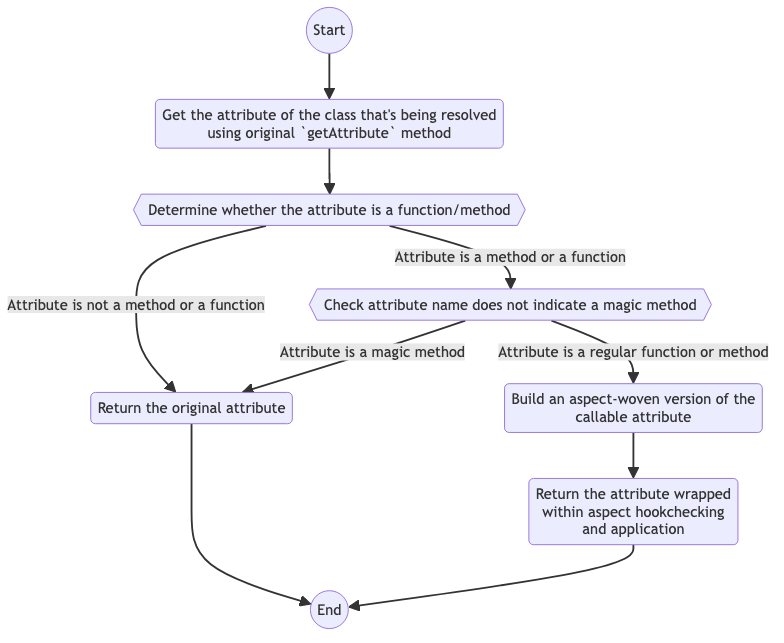
\includegraphics[width=0.9\columnwidth]{30_prior_work/diagrams/replacement_getattr.png}
\caption{High-level representation of the process implemented by the replacement
\lstinline{__getattribute__} method as implemented by the original \pdsf{}
library.}
\label{fig:early_pdsf_replaced_getattr_diagram}
\end{figure}

The replacement \lstinline{__getattribute__} method injected by
\pdsf{} also looks up attributes in the relevant object's underlying dictionary,
but in addition to retrieving an object's attribute it searches for advice to be
applied when performing these lookups, and applies any advice it finds. The
replaced attribute lookup logic implements the aspect hook woven by \pdsf{}.

Hooks are applied to a class by way of an invocation to a function,
\lstinline{fuzz_clazz}, which takes a class as a parameter and weaves aspect
hooks into that class~\cite{pdsf_repo,asp_repo}. \lstinline{fuzz_clazz} replaces
the \lstinline{__getattribute__} method of the class with a new function
object which it constructs. The replacement function object discovers aspects
which have been woven, invokes them, and also invokes the target of any woven
aspects at the correct time. Without any woven aspects, this has the effect of
simply executing a target function; however, in following this process the
replaced function object also implements aspect hooks.

The implementation of the function constructing the replaced attribute lookup
logic as well as the aspect hook implementation is given in
\cref{fig:weave_clazz_impl_early_pdsf}, which is edited slightly for legibility.
The replacement \lstinline{__getattribute__} method first makes a call to the
class' original \lstinline{__getattribute__} method to retrieve an attribute
when required. If this attribute is not a function or method, it is returned by
the woven \lstinline{__getattribute__} function and the affected class behaves
as if it was never altered. However, if an attribute to be retrieved is a method
or function, a new function is constructed and returned. This function contains
the aspect hooks described earlier. When it is invoked, the function retrieves
woven advice, invokes it at the appropriate points, and invokes the attribute it
replaced at the appropriate time. 

\begin{figure}[hp]
    \centering
    \lstinputlisting{30_prior_work/snippets/fuzz_clazz.py}
    \caption{The implementation of \lstinline{fuzz_clazz}, a function which
    replaces \lstinline{__getattribute__} on Python 2 objects to return
    callable attributes wrapped within an aspect hook implementation.}
    \label{fig:weave_clazz_impl_early_pdsf}
\end{figure}


\subsection{Applying Process Mutations}\label{subsec:prior_work_mutations}

The development of \pdsf{} was intended to support simulation \& modelling
research by providing a way of applying program modifications at runtime. It
sought to support models where a (potentially
non-deterministic) change to the behaviour was required, and enable
it to apply that change dynamically during execution in an \aspectoriented fashion.
\Aspectorientation{} libraries typically support advice woven before, around, or
after a join point; modifying the join point itself essentially allows changes
inside its definition, introducing a fourth type of weaving. \pdsf achieves this
through a special type of ``before''-style aspect termed a ``fuzzer''.

Fuzzers implement transformations on abstract syntax trees. They are implemented
as functions which receive a list of AST objects representing the body of a
function definition which matches a fuzzing advice's pointcut, and return
another list of AST objects, which replace the target function's definition. Any
transformation resulting in a valid AST is permitted. A code snippet
demonstrating the implementation of this process is shown in
\cref{fig:v1_pdsf_fuzzing_impl_codesnippet}, edited lightly for legibility.

\begin{figure}[hp]
    \centering
    \lstinputlisting{30_prior_work/snippets/FuzzingAspect.py}
    \caption{A code snippet from the original \pdsf implementation, implementing
    \lstinline{Fuzzing} aspects and applying fuzzing to a function definition.}
    \label{fig:v1_pdsf_fuzzing_impl_codesnippet}
\end{figure}

As can be seen in \cref{fig:v1_pdsf_fuzzing_impl_codesnippet}, fuzzing aspects
are implemented by way of ``prelude'' advice (\pdsf{} nomenclature for advice
run \emph{before} a target invocation, inspired by early work on \theatreag{},
which is discussed in \cref{subsec:prior_work_theatre}). Using prelude advice,
the \lstinline{apply_fuzzing} method is called before a target is invoked. This
method ensures that the correct function object and key to look up advice are
selected (which requires different logic depending on whether the target is a
method or a function), retrieves any advice woven onto to the target, and calls
the function \lstinline{fuzz_function} on it. Fuzzing is dynamically applied, as
advice is retrieved and applied only when a target is invoked and its prelude
advice is executed.

\lstinline{fuzz_function} retrieves the abstract syntax tree
(\emph{``AST''}) of the target, a tree representation of the Python code
implementing the target. This is cached in case fuzzing is applied to a target
multiple times, resulting in a changed AST every time. A copy is made, and a
\lstinline{WorkflowTransformer} recursively visits nodes of the AST and applies
the transformations defined by any discovered fuzzers to function definitions
within the AST. The implementation of a workflow transformer is given in
\cref{fig:workflowtransformer_implementation}. After transforming the AST, it is
compiled into a Python \lstinline{code} object and used to replace the code
object containing the target's implementation. This has the effect of changing
the behaviour of the target function, which now executes the program represented
by the transformed AST when it is invoked. As fuzzing is implemented as prelude
advice, this invocation is guaranteed to occur presently, meaning that the
transformation is guaranteed to occur right before the function is run. A fuzzer
transforming an AST can therefore make its transformations conditionally based
on the state of the program with little chance that the program state will
change afterward.\footnote{Later prelude advice or the initial stages of around
advice could theoretically also change program state, meaning programmers must
still be cautious about assumptions of program state.}

\begin{figure}[hp]
    \centering
    \lstinputlisting{30_prior_work/snippets/WorkflowTransformer.py}
    \caption{A code snippet from the original \pdsf implementation, implementing
    the \lstinline{WorkflowTransformer} which visits AST nodes and applies
    fuzzing to them.}
    \label{fig:workflowtransformer_implementation}
\end{figure}


\subsection{Limitations}\label{subsec:prior_work_pdsf_limitations}

The original implementation of \pdsf demonstrated the feasibility
of runtime metaprogramming as applied to simulation \& modelling.
However, its design presents limitations.

There is an overhead involved in running the wrapped
\lstinline{__getattribute__} function for every invocation of a fuzzed class,
and also in running aspect hooks for all possible join points even when those
hooks are not targets of advice at a given moment. When an attribute is the
target of advice, aspects are discovered and applied. However, aspects are
discovered by lookup within the scope of the function creating a replacement
\lstinline{__getattribute__} method. This design requires multiple instances
of advice weaving to create multiple replacement \lstinline{__getattribute__}
calls, all of which are invoked on any attribute lookup on a target class. A single target of
advice which has multiple pieces of advice woven therefore incurs a performance
penalty for every piece of advice applied, which must be incurred when any
attribute is looked up on the target's class. If the join point defining the
target may apply to many classes, each class must incur the same penalty, even
if none of their attributes are targets of advice in practice. The original
library was developed to demonstrate the feasibility of the idea underlying
\pdsf{} (runtime metaprogramming), but the weaving mechanism implemented left
room for improvement. A robust implementation with attention paid to reducing
this overhead is introduced in \cref{chap:pdsf_rewrite}.

Similarly, an additional overhead is incurred by a lack of caching of the
modifications fuzzers make to function definitions. One can envisage a need for
runtime metaprogramming which produces different function definitions at
different times: an example could be modelling different degrees of degraded
modes introduced to an actor's behaviour in safety-critical systems
research~\cite{johnson2007degradedmodes}. One can also envisage no such need: an
example could be minor temporary modifications otherwise permanently made in
program maintenance, such as to constants within a function definition, to the
format of a function's return value, or adding control flow which exits a
function early on a termination condition. The requirement is a product of the
tool's use case in different scenarios. In scenarios where the same modification
is to be made every invocation, a fuzzer need only be run once; optimisations
enabling the caching of fuzzing aspects' effects would provide better
performance in use cases where such a feature is appropriate.

Other aspect orientation frameworks offer support for other types of advice.
Handi-wrap and AspectJ both support features related to the processing of
exceptions thrown by a program~\cite{Baker_2002,aspectj_intro} and these
features have inspired work into improved exception handling in object-oriented
systems~\cite{millham2011aopandoopsecurity}. However, this version of \pdsf
offers no direct support for exception handling. Opportunities to support the
feature were therefore available for future revisions of the library to
capitalise on; such a revision is also presented in \cref{chap:pdsf_rewrite}.

A final limitation is that the weaving technique this early of \pdsf used is
incompatible with Python3, as replacing \lstinline{__getattribute__} is not
possible in Python's newer version. It was determined that a tool which was of
practical use to the simulation and modelling community should be produced which
would remain useful to future researchers making modern models; as the existing
weaving technique lacked performance, an opportunity presented itself for a
complete redesign. The resulting new design is presented in
\cref{chap:pdsf_rewrite} which makes use of a new weaving technique.



\section{Additional Simulation Machinery}\label{sec:prior_work_machinery}

Other related projects developed tooling for sociotechnical simulation \&
modelling. Fuzzi-Moss was a project collecting a library of standardised
behavioural modifications for use in sociotechnical simulation \& modelling;
\theatreag{} was a project offering a model of time against which actors within
sociotechnical simulations \& models could act. While these projects ultimately
were not used in producing the contributions of this thesis, they are outlined
here as relevant to the original \pdsf project as they were originally
developed as a suite of simulation \& modelling tools to be employed together.

\subsection{Fuzzi-Moss}\label{subsec:prior_work_fm}

Fuzzi-Moss\footnote{A backronym for ``Fuzzing Models of sociotechnical
simulations''} was a library of standard behavioural variations written as
fuzzers to be applied by \pdsf{}~\cite{fuzzimoss_repo}. It was primarily created
for use in a model of the impact of inconsistency in teams' executions of
software engineering methodology, which is discussed further in
\cref{sec:caise_paper}.

\begin{figure}
    \begin{lstlisting}
def missed_target(random, pmf=default_distracted_pmf(2)):
    """
    Creates a fuzzer that causes a workflow containing a while loop to be prematurely terminated before the condition
    in the reference function is satisfied.  The binary probability distribution for continuing work is a function of
    the duration of the workflow, as measured by the supplied turn based clock.
    :param random: a random value source.
    :param pmf: a function that accepts a duration and returns a probability threshold for an
    actor to be distracted from a target.
    :return: the insufficient effort fuzz function.
    """

    def _insufficient_effort(steps, context):

        break_insertion = \
            'if not self.is_distracted() : break'

        context.is_distracted = IsDistracted(context.actor.clock, random, pmf)

        fuzzer = \
            recurse_into_nested_steps(
                fuzzer=filter_steps(
                    fuzz_filter=include_control_structures(target={ast.While}),
                    fuzzer=recurse_into_nested_steps(
                        target_structures={ast.While},
                        fuzzer=insert_steps(0, break_insertion),
                        min_depth=1
                    )
                ),
                min_depth=1
            )

        return fuzzer(steps, context)

    return _insufficient_effort
    \end{lstlisting}
\end{figure}

Fuzzi-Moss contained utilities and fuzzers such as:

\begin{itemize}
    \item Two probability mass functions representing the chance that
    behaviour is to be altered given a length of time and an actor's\ldots{}:
    \begin{itemize}
        \item conscientiousness, a lack of which would increase chance of behavioural adaptation due to lack
    of effort;
        \item concentration, a lack of which would increase chance of behavioural
    adaptation due to distraction
    \end{itemize}
    \item A \lstinline{missed_target} fuzzer, which terminated a
    \lstinline{while} loop early if activated via a probability mass function of
    an actor's propensity for negligence. As an example of a Fuzzi-Moss fuzzer,
    this is shown in \cref{fig:fuzzimoss_missed_target_fuzzer}.\revnote{Consider
    moving some code snippets like those of Fuzzi-Moss, which aren't necessarily
    that important in the grand scope of the thesis, to an appendix.}
    \item An \lstinline{incomplete_procedure} fuzzer, which truncated the
    steps\footnote{Represented by lines of code} taken by an actor if activated
    via a probability mass function representing an actor's propensity for
    distraction
\end{itemize}

Plans were also made for fuzzers representing an actor ``becoming
muddled''\footnote{A behavioural variation caused by confusion.} and making
mistakes in decision-making, but neither have been completed at time of writing.
A discussion around the revival of this project in the context of the \pdsf
rewrite presented in \cref{chap:pdsf_rewrite} is given in
\cref{future_work_revive_fuzzimoss}. 


\subsection{\theatreag{}}\label{subsec:prior_work_theatre}

\theatreag{} is a project defining a model of time against which actors in
sociotechnical models \& simulations can act~\cite{theatre_ag_repo}. In the
project's overview, it describes itself as\ldots{}:

\begin{blockquote}
    \theatreag{} is a workflow oriented agent based simulation environment.
    \theatreag{} is designed to enable experimenters to specify readable workflows
directly as collections of related methods organised into Plain Old Python
Classes that are executed by the agents in the simulation. All other simulation
machinery (critically task duration and clock synchronization) is handled
internally by the simulation environment.
\end{blockquote}

The central metaphor underlying \theatreag{}'s model of timing is theatrical: actors
in a simulation or model are members of a ``cast'' (a collection of actors) who
enact a ``workflow'' (simulation steps) in a ``scene'' (domain model within
which the actors interact). Central to the library is its clock: tasks are given
durations, and a clock which synchronises all agents' position in time ticks to
complete different tasks. The theatrical model \theatreag{} introduces is the context
for \pdsf{}'s nomenclature for its types of advice: ``prelude'' advice happens
before a task and ``encore'' advice is invoked afterward as a prelude and
encore would be in a literal theatre.

\theatreag{} has been used as the environment in models of TCP/IP, algorithmic
trading, the spread of disease~\cite{aranTheatreThesis}, and the impact of
behavioural variation in software engineering methodologies as described in
\cref{sec:caise_paper}.


\section{Example Studies using \pdsf for Behavioural Simulation}\label{sec:caise_paper}

The viability of encoding behavioural variations as aspects using \pdsf has been
demonstrated in earlier studies~\cite{wallis2018caise,aranTheatreThesis}.
\revnote{Maybe I should include something on Aran's master's dissertation too,
rather than just citing it?} The study modelled software engineers working to
different methodologies of software engineering: waterfall, in which
requirements are gathered, software is developed to meet requirements, quality
assurance steps are undertaken, and the resulting software is delivered to
customers; and TDD, where the development of tests for quality assurance
precedes the development of features. The study sought to investigate whether,
when software engineers were working suboptimally, there was a difference in the
rate of bugs introduced to a program developed under each methodology.

The study began with a ``naive'' model of software engineers following each
paradigm, developed in Python using \pdsf{}, \theatreag{}, and Fuzzi-Moss. Engineers
would produce ``chunks'' of code, which could contain bugs. In quality
assurance, engineers were modelled as attempting to identify bugs in different
areas of the codebase, fixing them if they were discovered. Developers could
commit chunks of code toward features identified through requirement
engineering, which were eventually completed, but could potentially contain
undiscovered bugs within chunks of code.

This model was then augmented aspectually using \pdsf{}. Distraction was
represented through the truncation of functions representing workflow steps.
Developers were modelled with different levels of distraction, affecting a
probability mass function (PMF) which would activate when a developer was
modelled as being distracted in a given moment. If the PMF activated, the
workflow step invoked at that moment was truncated using \pdsf{}. The model showed
that developers following the TDD methodology could successfully complete a
larger number of features on average than those following waterfall, concurring
with the prevailing consensus on the two methodologies. \revnote{Add a citation
for TDD vs agile! Citations are missing from the copy of the CAiSE paper I can
find, but I'd like to use the same one.}

In replicating the community understanding of the model, the paper demonstrated
the feasibility of aspectually augmenting modelled behaviour: the simulation
took a naive model with no capacity for analysing errors, and introduced new
features of the model supporting an avenue of investigation otherwise
impossible with the methodologies represented by the naive model. That the
resulting simulation matched the expectations existing within the community gave
confidence that the tool could be used to build realistic simulations where
some features of a model could be separated from its core codebase.

\inline{
  If there's time, add a section on Aran's thesis specifically (if not don't
  worry --- it's cited elsewhere in this chapter)
}

\section{Discussion}\label{sec:prior_work_discussion}

The existing case study employing \pdsf demonstrated that realistic model
features could be separated from their core codebase, and gave credence to
\pdsf{}'s use as a tool for aspectually augmenting models with behavioural
variance. It also left many research questions unanswered and tooling
flaws unsatisfied, however:\revnote{Does this want to be a list? Consider
reworking to a paragraph.}

\begin{itemize}
    \item Aspects were believed to be ``realistic'' as they represented the
    expected outcomes of the simulation. However, no real-world data was used to
    corroborate the claim, and it was unclear that aspectually augmented
    behaviour could capture the variations present in real-world human
    behaviour.
    \item These aspects also demonstrated variations which were identifiable in
    the emergent properties of a system (for example, mean time to failure of a
    software system under development, or successfully completed features). The
    variations applied to individual developers might have poorly modelled
    individual behaviour, but produced accurate emergent properties of the
    system individual developers acted within.
    \item As discussed in \cref{subsec:prior_work_pdsf_limitations}, \pdsf's
    implementation at the time was a proof-of-concept which, while successfully
    demonstrating the potential of aspect-oriented runtime metaprogramming, was
    also inefficient, feature-incomplete, and lacked compatibility with modern
    software engineering tooling.
    \item Models of distraction were adopted from the common library provided by
    Fuzzi-Moss. However, this model was not applied to other codebases. It
    remains unclear that Fuzzi-Moss' model of distraction is broadly applicable
    in other projects: different models of distraction might be required by
    different researchers. Further, a model of distraction which realistically
    represents the behaviour of an individual (rather than the emergent
    properties of the system that individual acts within) might not apply to
    other systems the individual acts within. Briefly put, The portability of
    aspectually modelled behavioural simulation has not been investigated, and
    literature within the aspect orientation community lacks evidence to support
    a belief in their portability~\cite{przybylek2010wrong,Constantinides04aopconsidered,steimann06paradoxical}.
\end{itemize}

This leaves opportunities to improve both the tooling offered for aspect-oriented
runtime metaprogramming, and the evidence supporting its use to encode
behavioural variations in sociotechnical systems. Improvements to the tooling
follow in \cref{chap:pdsf_rewrite}; later chapters propose --- and discuss the
implementation of --- real-world systems which are suitable for modelling using
\pdsf{} in \cref{chap:rpglite}, and a study of those systems using aspectually
augmented models in \cref{chap:exp1_simulation_optimisation} and \cref{chap:exp2_old_aspects_new_systems}.
